% slides.tex 
% ICMC 2002 slides 
%**start of header
\documentclass{slides}
\usepackage{amsmath,amssymb,amscd,epsfig}
%\usepackage{times}
\usepackage{theorem}
\onlyslides{1-100}
%\usepackage{fullpage}
\usepackage{ifthen}

%% Should figures be compiled?
\newboolean{nofigures} % initially false ==> compile with figures
% comment out the following line to compile without figures
%\setboolean{nofigures}{true} 

\newboolean{notable}
\setboolean{notable}{true} 
\newboolean{noambiguity}
\setboolean{noambiguity}{true} 
\newboolean{noearlierwork}
%\setboolean{noearlierwork}{true} 
%
%-------------------------------------------------------------
%
\thispagestyle{empty}
\newcommand{\HRule}{\rule{\linewidth}{.05mm}}
%\setlength{\parindent}{0mm}
%\setlength{\parskip}{0mm}

\def\HOME{/home/sonic/pub/research/dsp/DeMeo/notes}
\def\R{\mathbb{R}}    % real numbers 
\def\Z{\mathbb{Z}}    % real numbers 
\def\C{\mathbb{C}}    % complex numbers 
\def\e{\mathrm{e}}    % exponential
% Two notations for real part of a complex number
   \def\Real{\mbox{Re}}  %\def\Real{\Re}
% Two notations for integration over R
   \def\integral{\int_{-\infty}^{\infty}}
     %\def\integral{\int_{-\infty}^{+\infty}} 
% Operator Theory
   \def\A{\operatorname{A}}
   \def\E{\operatorname{E}}
   \def\H{\operatorname{H}}
%   \def\I{\operatorname{I}}
   \def\P{\operatorname{P}}
   \def\pv{\operatorname{pv}}
   \def\S{\operatorname{S}}
   \def\T{\operatorname{T}}
   \def\W{\operatorname{W}}
   \def\Hilbert{\mathcal{H}}
   \def\Hone{\mathcal{H}_1}
   \def\Htwo{\mathcal{H}_2}
   \def\Banach{\mathcal{B}(\Hilbert,\Hilbert)}
   \def\Banachonetwo{\mathcal{B}(\Hone,\Htwo)}
   \def\Banachtwoone{\mathcal{B}(\Htwo,\Hone)}
   \def\Lone{L^1}
   \def\Ltwo{L^2}
   \def\ltwo{\ell^2}
   \def\LoneR{L^1(\mathbb{R})}
   \def\LtwoR{L^2(\mathbb{R})}
   \def\ltwoR{\ell^2(\mathbb{R})}
   \def\Null{\mathcal{N}}  % nullspace
% Signals, Time-Frequency shifts, etc.
   \def\scale{\frac{1}{\sqrt{s}}}
   \def\transcale{\left(\frac{t-u}{s}\right)}
   \def\xpull{x_{\frac{\tau}{2}, -\frac{\xi}{2}}}
   \def\xpush{x_{-\frac{\tau}{2}, \frac{\xi}{2}}}
   \def\xpullpush{x_{\frac{\tau}{2}, \frac{\xi}{2}}}
   \def\xpushpull{x_{-\frac{\tau}{2}, -\frac{\xi}{2}}}
   \def\xfpull{x_{-\frac{\Delta\nu}{2}}}
   \def\xfpush{x_{\frac{\Delta\nu}{2}}}
   \def\apull{a_{-}}
   \def\apush{a_{+}}

   \def\ytnu{y_{t,\nu}}
   \def\ytnut{\tilde{y}_{t,\nu}}
   \def\half{{\scriptstyle \frac{1}{2}}}
   \def\halftau{{\scriptstyle \frac{\tau}{2}}}
   \def\halfxi{{\scriptstyle \frac{\xi}{2}}}
   \def\halfnu{{\scriptstyle \frac{\nu}{2}}}
   \def\halfDnu{{\scriptstyle \frac{\Delta\nu}{2}}}

   \def\xtpull{x\left(t+\halftau\right)}
   \def\xtpush{x\left(t-\halftau\right)}
%   (shouldn't need this) \def\xtpullconj{x^*\left(t+\halftau\right)}
   \def\xtpushconj{x^*\left(t-\halftau\right)}
   \def\Xtpull{X\left(\nu+\halfxi\right)}
   \def\Xtpush{X\left(\nu-\halfxi\right)}
   \def\Xtpullconj{X^*\left(\nu+\halfxi\right)}
%   (shouldn't need this) \def\Xtpushconj{X^*\left(\nu-\halfxi\right)}

   \def\ytpull{y\left(t+\halftau\right)}
   \def\ytpush{y\left(t-\halftau\right)}
%   (shouldn't need this) \def\ytpullconj{y^*\left(t+\halftau\right)}
   \def\ytpushconj{y^*\left(t-\halftau\right)}
   \def\Ytpull{Y\left(\nu+\halfxi\right)}
   \def\Ytpush{Y\left(\nu-\halfxi\right)}
   \def\Ytpullconj{Y^*\left(\nu+\halfxi\right)}
%   (shouldn't need this) \def\Ytpushconj{Y^*\left(\nu-\halfxi\right)}

\def\a{\mathbf{a}}
\def\b{\mathbf{b}}

% Language
   \def\FT{Fourier transform}
   \def\WT{Wigner transform}
   \def\WV{Wigner-Ville}

\begin{document}
\HRule\\\\
%\begin{flushleft}
%        \Huge Postmusic\\[5mm]
%        \Large Technical Report: \large rhythm and pitch
{\Large {\tt Characterizing musical signals}}\\\\
{\Large {\tt with Wigner-Ville interferences}}\\
%\hspace*{\stretch{1}} 17 September 2002
%\end{flushleft}
\HRule
%\begin{center}
\begin{center}
\begin{tabular}{rcl}
William DeMeo &\hspace{2cm}& {\tt williamdemeo@yahoo.com}\\
\\
{\small ICMC 2002}&\hspace{2cm}& {\small G\"{o}teborg, Sweden}
\end{tabular}\\
\vspace{4cm}
{\tt www.harmonicanalysis.com}\\
{\tt www.incunabula.us}
\end{center}

%%% Slide 1
\begin{slide}
\begin{center}{\tt \underline{OUTLINE}}\end{center}
\begin{enumerate}
\item 
{\it Musical Signal Decomposition}\\
find representation which facilitates a\\
measure of perceived qualities.

Review well-known decomposition 
method: ``matching pursuit.''

\item 
{\it Perceived Qualities}\\
$\cdot$ melodic dissonance\\
$\cdot$ sensory dissonance 
\item 
{\it Wigner-Ville interference}\\
specious signal energy or
revealing of \\ 
perceived qualities?

\end{enumerate}
\end{slide}

\ifthenelse{\boolean{noearlierwork}}{}{
\begin{slide}%%% Slide 
\begin{center}{\tt \underline{PREVIOUS WORK}}\end{center}
{\bf consonance/dissonance analysis}\\
%\begin{itemize}
$\cdot$ Helmholtz, {\it On the Sensation of Tone}, 1877.\\
$\cdot$ Plomp \& Levelt, %{\it Tonal Consonance and Critical Bandwidth}, 
JASA 1965.\\
$\cdot$ Sethares, %{\it Tuning, Timbre, Spectrum, Scale}, 
Springer 1997.\\
\\
%\end{itemize}
{\bf matching pursuit decomposition}\\
%\begin{itemize}\item 
$\cdot$ Mallat \& Zhang, %{\it Matching Pursuits with Time-Frequency Dictionaries},
IEEE Trans SP, 1993.\\
$\cdot$ Gribonval, Depalle, Rodet, Bacry, Mallat, \\
%{\it Sound signal Decomposition using high resolution matching pursuit}, 
ICMC Proceedings, 1996.\\
\\
%\end{itemize}
{\it et} many {\it al}...
\end{slide}
}

\begin{slide}%%% Slide 
\begin{center}{\tt \underline{INTRODUCTION}}\end{center}
Let $x(t)$ be a musical signal.  Measure ``dissonance'' of $x$ at time 
instant $t = t_i$ as a function of estimated frequency components of $x$ at
$t_i$.  
\begin{align*}
D(t_i) &= \text{ dissonance of } x \text{ at } t_i\\
&= \text{ fn of frequencies at } t_i\\
&= D(t_i, \alpha_0, \alpha_1,\ldots)
\end{align*}
Can account for ``instantaneous'' dissonance.\\
Cannot account for melodic contour.
\end{slide}

\begin{slide}%%% Slide 
\begin{center}{\tt \underline{PERCEIVED QUALITIES}}\end{center}
\begin{itemize} 
\item {\bf Melodic Consonance (CDC-1):} \\
depends on melodic context; must be fn of $x(t_i)$ as well as 
$x(t_j)$ for $j \neq i$; accounts for relations among pitches sounded at
different times. 
\item {\bf Sensory Consonance (CDC-5):} \\
equates consonance with smoothness/absence of beats;
dissonance with roughness/presence of beats;
accounts for relations among pitches sounded simultaneously.
\end{itemize} 
\end{slide}

\begin{slide}%%% Slide 
\begin{center}{\tt \underline{TIME-FREQUENCY REPRESENTATION}}\end{center}
{\bf Wigner-Ville Transform (WVT)}:\\
correlates a signal with a time and frequency
shifted version of itself.\\
\begin{equation*} %\label{eqn:WignerVille}
\W_x(t,\nu) = 
\int \xtpull \xtpushconj e^{-i2\pi \tau\nu}\,d\tau
\end{equation*}
\\
It is the \FT\ of
\[
\phi_x(t,\tau) = \xtpushconj \xtpull
\]
\end{slide}

\begin{slide}%%% Slide
%The WVT localizes the time-frequency structures of $x$.  
{\bf Covariance Property:} \\
If energy of $x$ is concentrated around $(t_0,\nu_0)$, then energy of $\W_x$ is centered at
$(t_0,\nu_0)$ with time-frequency spread equal to that of $x$.  \\
\\
%\begin{center}{\tt \underline{}}\end{center}
{\bf Cross \WV\ Transform:} %of $x$ and $y$
\[
  \W_{xy}(t,\nu) = \int \xtpull \ytpushconj e^{-i2\pi\nu\tau}\,d\tau 
\]
\[
  \W_{yx}(t,\nu) = \int \ytpull \xtpushconj e^{-i2\pi\nu\tau}\,d\tau 
\]
\end{slide}

\ifthenelse{\boolean{noambiguity}}{}{
\begin{slide}%%% Slide 
{\bf Ambiguity Function (AF):}
%The \emph{ambiguity function} (AF) is
\[
\A_{x}(\xi,\tau) = \int \xtpull \xtpushconj e^{i2\pi \xi t}\,dt
\]
\\
WVT is 2-d Fourier transform of AF.
\[%\begin{equation}\label{eq:ambig-ft}
\W_x(t,\nu) = 
  \iint%\limits_{\R^2} 
    \A_x(\xi,\tau) e^{-i2\pi(\xi t + \nu\tau)}\,d\xi\,d\tau
\]%\end{equation}
\end{slide}
}

\begin{slide}%%% Slide 
\begin{center}{\tt \underline{INTERFERENCE STRUCTURE}}\end{center}
WVT does not conform to linear superposition; instead,
\begin{align*}
  \W_{x+y}(t,\nu) &= \W_x(t,\nu) + \W_y(t,\nu)\nonumber \\
      \quad &+ \W_{xy}(t,\nu) +\W_{yx}(t,\nu)
\end{align*}
%where $\W_{xy}$ is the cross WVT of $x$ and $y$.\\
%\\
%Similar to familiar quadratic expansion,\\
%$(a+b)^2 = a^2 + b^2 + ab + ba$\\
\\
%\end{slide}
%\begin{slide}%%% Slide 
{\bf Interference term:}
\begin{align*}
  I_{xy}(t,\nu) &= \W_{xy}(t,\nu) + \W_{yx}(t,\nu)\\
                &= 2\,\Real\left[\W_{xy}(t,\nu)\right]
\end{align*}
creates non-zero values at
interesting locations of the time-frequency plane. 
\end{slide}

\begin{slide}%%% Slide 
More generally, the composite signal
\[
  x(t) = \sum_{n=1}^N a_n x_n(t)
\]
\\
has WVT
\begin{align*}
  \W_{x}(t,\nu) &= \sum_{n=1}^N|a_n|^2 \W_{x_n}(t,\nu) \\ %\label{eq:WignerSum} \\
\\
 &+ 2\sum_{n=1}^{N-1}\sum_{k=n+1}^N\,
                 \Real\left[a_n a_k^* \W_{x_nx_k}(t,\nu)\right]
\end{align*}
%\\
%For a composite signal with $N$ components
%we must compute $N(N-1)/2$ cross terms.
\end{slide}

\begin{slide}%%% Slide
\begin{center}{\tt \underline{WEYL-HEISENBERG OPERATOR}}\end{center}
Consider elementary signal $x \in L(\Z/N)$\\
$\cdot$ discrete, periodic function with period $N$,\\
$\cdot$ defined on group $\Z/N \simeq \{0,1,\ldots,N-1\}$.\\
\\
{\bf Weyl-Heisenberg operator:}\\
Define $H : \Z /N \times \Z /N \rightarrow  L(\Z /N)$ by
%is defined by
\begin{align*}
H(\a)x(n) &= x_\a(n) \nonumber\\
&= x(n-a_1)\;e^{i2\pi a_2n/N}
%\; x \in L(\Z/N) %\label{eqn:transmod}
\end{align*}
for any $\a = (a_1,a_2) \in \Z /N \times \Z /N$.
\end{slide}

\begin{slide}%%% Slide
\begin{center}{\tt \underline{EXAMPLE}}\end{center}
Let %$x$ be pure sinusoidal
$x(t) = e^{i2\pi\nu_m t}$
\[\a = (0,-\halfDnu)\; \Rightarrow\;
x_\a(t)=e^{i2\pi(\nu_m-\halfDnu)t}\]
%at (mid-point) frequency $\nu_m$.\\
%Let $\a = (0,-\halfDnu)$, $\b = (0,\halfDnu)$.
\[
 \b = (0,\halfDnu) \;\Rightarrow \;x_\b(t)= e^{i2\pi(\nu_m+\halfDnu)t}
\]\\
Composite signal is 
\begin{align*}
%=e^{i2\pi(\nu_m-\halfDnu)t}+e^{i2\pi(\nu_m+\halfDnu)t}\\
x_\a(t) + x_\b(t) &= 2\cos(2\pi \halfDnu t)\, e^{i2\pi\nu_mt}
\end{align*}
%\\
%Notation: $x_{\a \b}(t) = x_\a(t) + x_\b(t)$.
\end{slide}
\begin{slide}
{\bf PHYSICAL INTERPRETATION:}\\
%Relate this to physical phenomenon of
%beats, perceived most easily when distance between
%signal components is small.  
Composite signal has WVT 
\begin{align*}
 \W_{x_{\a \b}}(t,\nu)&=\delta(\nu-(\nu_m-\halfDnu))+\delta(\nu-(\nu_m+\halfDnu))\\
\\
&\quad +\delta(\nu-\nu_m)\,2\cos(2\pi \Delta\nu t)
\end{align*}\\
When components $x_\a(t)$ and $x_\b(t)$ are close in
frequency, % that is, when $\Delta\nu$ is small -- the 
cosine term is slowly varying. \\
\\
%as compared to exponential term,
Composite signal %can be viewed as 
viewed as simple tone with \\
$\cdot$ frequency $\nu_m$,\\
%slowly varying 
$\cdot$ modulated amplitude envelope, \\
$\cdot$ modulation frequency $\Delta\nu$.\\
``beats'' refer to such amplitude modulations. % due to interaction of signal components.
%Compare with following representation
%\begin{align*}
%x_{\a \b}(t) &=\half \,e^{i2\pi(\nu_m-\halfDnu)t} + \half \,e^{i2\pi(\nu_m+\halfDnu)t}\nonumber\\
%\\ &\quad + \cos(2\pi\halfDnu t)\,e^{i2\pi\nu_m t}\end{align*}
\end{slide}
%\begin{slide}
%\begin{center}{\tt \underline{BEATS}}\end{center}
%\end{slide}
%Comparing~(\ref{eq:sigbeats}) with~(\ref{eq:WignerBeats}), it is
%clearly the interference term of the \WT\ which specifies
%the existence and nature of beats in the composite signal.
% of interacting signal components.
\def\Per{\ensuremath{\operatorname{Per}}}
\begin{slide}%%% Slide
\begin{center}{\tt \underline{MATCHING PURSUIT (MP)}}\end{center}
Mallat \& Zhang, {\it Matching Pursuits with Time-Frequency Dictionaries},
IEEE Trans.~SP, 1993.

MP decomposes signal over elements of dictionary 
$\mathcal{D}= \{g_\gamma\}_{\gamma\in\Gamma}$.

{\bf MP Dictionary:}\\
Start with Gaussian window 
\[
f(t) = 2^{1/4}e^{-\pi t^2}
\]
Dictionary comprises periodic, scaled, \\
translated, and modulated versions of $f$.
\end{slide}

\begin{slide}%%% Slide
%{\bf Periodize:}
$\Per_{B}f$ denotes \emph{periodization} of $f$ over $B$.\\
%\[\Per_{B}f(a) = \sum_{x\in B} f(a+x), \quad a \in A\]
%$\Per _Bf$ is $B$-periodic.\\
\\
For $n \in \Z$ define discrete $N$-periodic window
\[
g(n) = \Per _{N\Z}f(n) = \sum_{m\in N\Z} f(n+m)
\]

Scaling by $s$,
\[
g_s(t) = \frac{1}{\sqrt{s}}g\left(\frac{t}{s}\right)
\]
\end{slide}
\begin{slide}%%% Slide
%\begin{center}{\tt \underline{}}\end{center}
Let $\gamma = (s, a_1, a_2)$ where
\begin{align*}
s &= \text{ scaling factor }\\
a_1 &= \text{ time translation}\\
a_2 &=\text{ frequency modulation}
\end{align*}
\begin{align*}
g_\gamma(t) &= g_s(t-a_1)\langle t,a_2 \rangle\\
\\
&= \frac{1}{\sqrt{s}}g\left(\frac{t-a_1}{s}\right) e^{i2\pi a_2 t}
\end{align*}
\\
$g_\gamma(t)$ defines a typical atom in the dictionary, with
energy %is centered at the abscissa $a_1$.  Its energy 
concentrated in a neighborhood of $(a_1,a_2)$, whose size is proportional
to $s$.
\end{slide}

\begin{slide}%%% Slide
\begin{center}{\tt \underline{}}\end{center}
Let discrete signal $x$ have length $N = 2^{K+1}$. \\
\\
Select dictionary parameters as follows:
\[
s = 2^j, \qquad j \in \{1,2,\ldots,K\}
\]
%Translation parameters are
\[
a_1 \in L_1\Z/N, \qquad L_1 = 2^{j-1}
\]
where
\begin{align*}
L_1\Z/N &= \{0, L_1, 2L_1, \ldots, (M_1-1)L_1\}\\
\text{and }\qquad N &= L_1M_1
\end{align*}

$\therefore$ translations separated by $\frac{s}{2} = 2^{j-1}$ samples.
\end{slide}
\begin{slide}
Suppose modulation parameters are
\[
a_2 \in M_1\Z/N = (L_1\Z/N)_*
\]
then $(a_1,a_2)$ ranges over
\[
L_1\Z/N \times M_1\Z/N = L_1\Z/N \times (L_1\Z/N)_*
\]
%modulation parameters $a_2$ are separated by $M_1$ samples, 
a \emph{critical sampling subgroup} of $\Z/N \times \Z/N$.  

Instead choose $M_2= 2^{K-j}$, and let $(a_1,a_2)$ range over
\emph{integer oversampling subgroup}
\[
\Delta_s = L_1\Z/N \times M_2\Z/N
\]
\end{slide}
\begin{slide}
%Define\[(x_1,x_2) &\in \{0,1,\ldots,M_1-1\} \times \{0,1,\ldots,L_2-1\}\]
%Translation-modulation pair is $(a_1,a_2) = (x_1L_1,x_2M_2)$.
{\bf Weyl-Heisenberg (W-H) system:}\\
For each $s$, $\langle g_s,\Delta_s \rangle$ defines a Weyl-Heisenberg system.

To the set of $K$ W-H systems add\\
$\cdot$ complex exponentials (Fourier basis)\\
$\cdot$ $N$ discrete Diracs
\end{slide}
\begin{slide}
{\bf Matching Pursuit (MP)}\\
iteratively decompose signal over $\mathcal{D}$ as follows:
\begin{enumerate}
\item set $R^0x(t)=x(t)$; assume $R^nx$ computed.
\item choose $g_{\gamma_n}$ which ``matches'' $R^nx$:
\[
|C(R^nx,g_{\gamma_n})| = \sup_{\gamma \in \Gamma} |C(R^nx,g_\gamma)|
\]
\item decompose residue $R^nx$ as
\[
R^nx(t) = C(R^nx,g_{\gamma_n})g_{\gamma_n}(t) + R^{n+1}x(t)
\]
\item repeat from step 2.
\end{enumerate}
\end{slide}
%\begin{slide}
%%$C(R^nx,g_\gamma)$ is a ``correlation'' function.
%$C$ is a ``correlation'' function.  For usual inner product
%$C(R^nx,g_{\gamma_n}) = \langle R^nx,g_{\gamma_n}\rangle$
%one can show 
%\[
%\|R^nx\| \downarrow 0\;\text{ exponentially with } n
%\]
%\end{slide}
\begin{slide}
$C$ is a ``correlation'' function.  For usual inner product
$C(R^nx,g_{\gamma_n}) = \langle R^nx,g_{\gamma_n}\rangle$
one can show 
\[
\|R^nx\| \downarrow 0\;\text{ exponentially with } n
\]\\
MP results in decomposition
\[
x(t) = \sum_{n=0}^\infty \langle R^nx,g_{\gamma_n} \rangle g_{\gamma_n}(t) 
\]
with WVT %\WV\ representation
\begin{equation*}
W_x(t,\nu) = \sum_{n=0}^\infty 
    \left|\langle R^nx,g_{\gamma_n} \rangle \right|^2 
\W_{g_{\gamma_n}}(t,\nu)\;+
\end{equation*}
\begin{equation*}
\sum_{m,n}
\langle R^mx,g_{\gamma_m}\rangle \langle R^nx,g_{\gamma_n}\rangle^*
\W_{g_{\gamma_m}g_{\gamma_n}}(t,\nu)
\end{equation*}
\end{slide}

\begin{slide}
%However, in at least that part of the literature dealing with musical signals,
%e.g.~Gribonval, {\it et al.} \citeyear{Gribonval:1996}, as well as more
%generally, we consistently find that the signal energy is reduced to
Most studies define signal energy as
\[
E_x(t,\nu) = \sum_{n=0}^\infty 
    \left|\langle R^nx,g_{\gamma_n}\rangle\right|^2 \W_{g_{\gamma_n}}(t,\nu) 
\]
\\
$\cdot$ only 1st term of WVT appears; \\
$\cdot$ assumption: 1st term accounts for energy of ``true'' signal components.

For $W_x(t,\nu)=E_x(t,\nu) +I_x(t,\nu)$ we define 
\begin{align*}
E_x(t,\nu) &= \text{ ``signal energy''} \\
I_x(t,\nu) &= \text{ ``interference energy''}
\end{align*}
%the cross terms of WVT by $I_x(t,\nu)$
\end{slide}
\begin{slide}%%% Slide
%\begin{center}{\tt \underline{}}\end{center}
Cost to compute cross WVT %among two time-frequency
roughly same as cost to compute WVT.

For a $N$-atom MP, must compute $N(N-1)/2$ cross WVT's.

Assuming:\\
$\cdot$ fast implementation based on FFT \\
$\cdot$ MP expansion has fewer than 1000's of atoms\\
$\Rightarrow$ computational burden still ``manageable.''
\end{slide}
\begin{slide}%%% Slide
\begin{center}{\tt \underline{EXAMPLE}}\end{center}
Construct signal by adding constant tone to ``linear chirp.''

Start at equal frequencies; chirp frequency increases linearly until double
that of constant tone. 

Demonstrates how constant tone interacts with frequencies 
in the octave above it.
%The research cited in the introduction (\citeN{Plomp:1965}, \citeN{Sethares:1997})
%suggests that we should expect the dissonance between two tones to be 0 when
%the two tones have the same frequency; the dissonance should then increase to
%a maximum, occuring when the tones are distinct but close in frequency, and
%then decrease as the difference in frequency between the tones increases.
\end{slide}

%%%%%%% FIGURES %%%%%%%%%%%
\ifthenelse{\boolean{nofigures}}{}{
\begin{slide}
  \begin{center}
  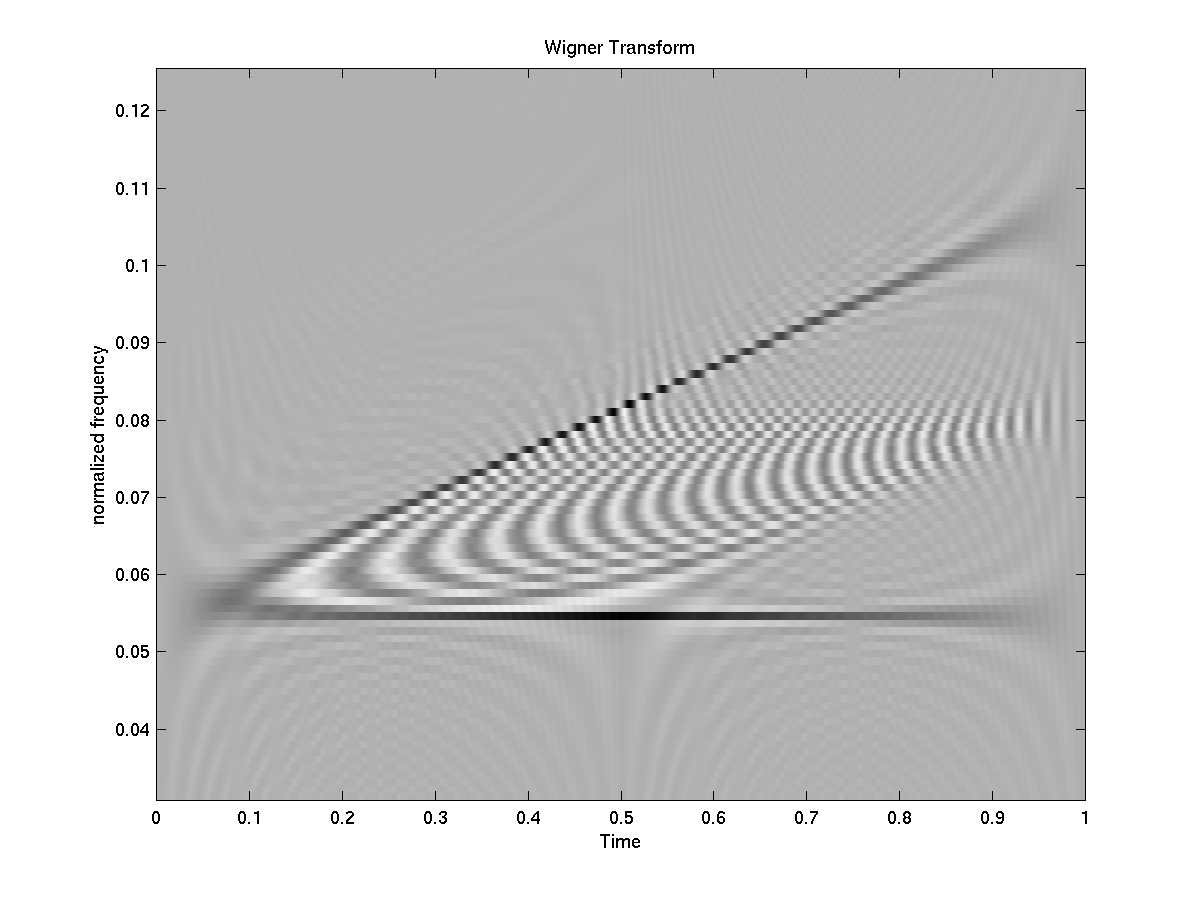
\includegraphics[width=14cm, height=10cm]{WVT}
  \end{center}
  WVT of constant frequency modulation plus linear chirp.
\end{slide}
\begin{slide}
  \begin{center}
  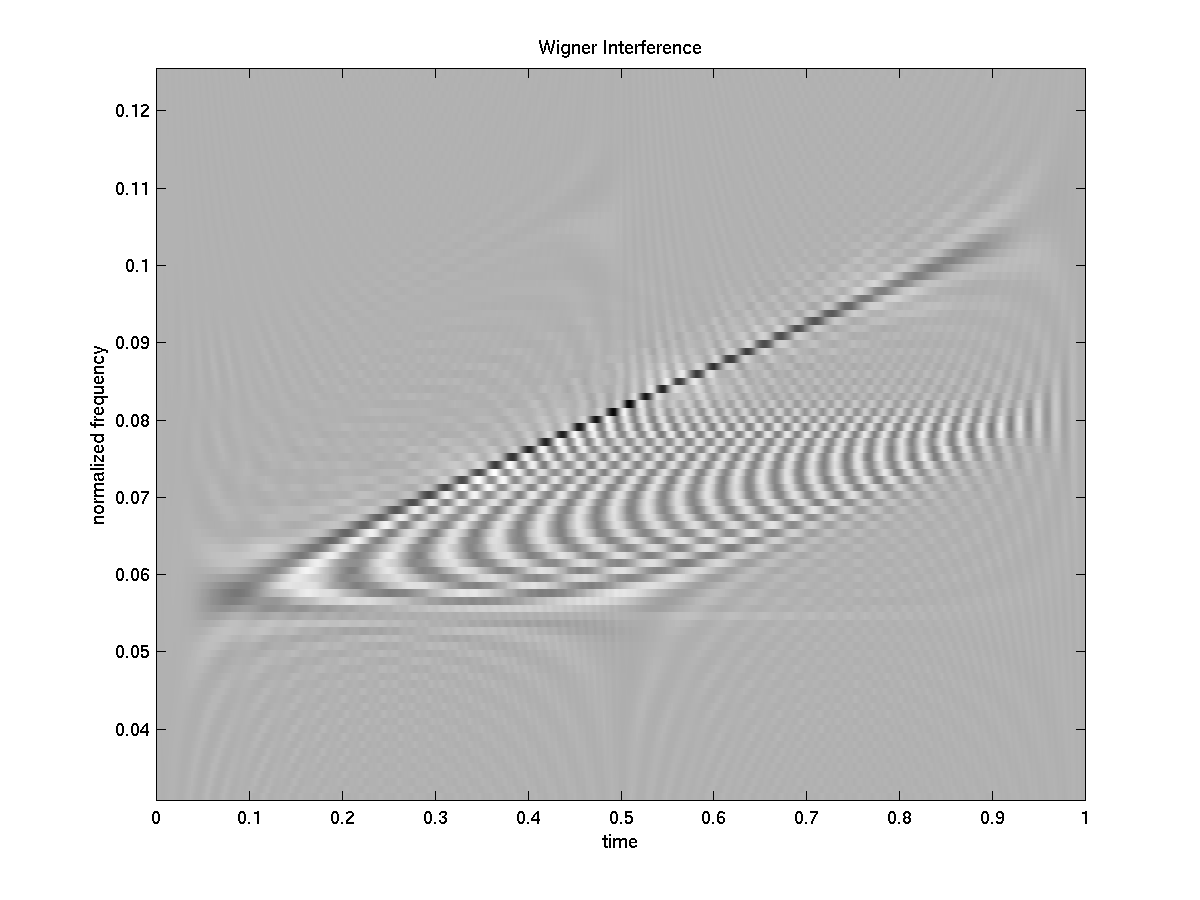
\includegraphics[width=14cm, height=10cm]{WVI}
  \end{center}
  Interference energy of constant frequency modulation plus linear chirp.
\end{slide}
}

\def\tpull{\left(t+\halftau\right)}
\def\tpush{\left(t-\halftau\right)}
\def\I{\mathcal{I}}
\begin{slide}%%% Slide
\begin{center}{\tt \underline{DISSONANCE MEASURES}}\end{center}
%More general definition of $\phi_x(t,\tau)$,
Define
\[
\phi_{g_{\gamma_m}g_{\gamma_n}}(t,\tau) 
= g_{\gamma_m}\tpull g^*_{\gamma_n}\tpush
\]\\
%By definition of cross WVT 
$\W_{g_{\gamma_m}g_{\gamma_n}}$ is Fourier transform
of $\phi_{g_{\gamma_m}g_{\gamma_n}}(t,\tau)$

$\therefore$ inverse FT of $\W_{g_{\gamma_m}g_{\gamma_n}}$ is
$\phi_{g_{\gamma_m}g_{\gamma_n}}$
\\
\[
\phi_{g_{\gamma_m}g_{\gamma_n}}(t,\tau) = \int
\W_{g_{\gamma_m}g_{\gamma_n}}(t,\nu) e^{i2\pi\nu\tau}\;d\nu
\]
\end{slide}

\begin{slide}%%% Slide
Integrating $\W_{g_{\gamma_m}g_{\gamma_n}}(t,\nu)$ over all $\nu$ is
equivalent to evaluating $\phi_{g_{\gamma_m}g_{\gamma_n}}$ at $\tau = 0$
\begin{align*}
\int
\W_{g_{\gamma_m}g_{\gamma_n}}(t,\nu)\;d\nu
&=\phi_{g_{\gamma_m}g_{\gamma_n}}(t,0)\nonumber \\
&= g_{\gamma_m}(t)g^*_{\gamma_n}(t) % \label{eq:intWV}
\end{align*}\\
{\bf 1st Dissonance Measure:} \\
``instantaneous interference''
% dissonance at $t$ of
%signal $x$ by integrating %interference energy
%$I_x(t,\nu)$ over all %frequencies 
%$\nu$.
\[
\I_x(t) = \int I_x(t,\nu)\; d\nu
\]
\[
=\sum_{m, n}
    \langle R^mx,g_{\gamma_m}\rangle \langle R^nx,g_{\gamma_n}\rangle^*
      \int \W_{g_{\gamma_m}g_{\gamma_n}}(t,\nu)\; d\nu
\]
\[
=\sum_{m, n}
    \langle R^mx,g_{\gamma_m}\rangle \langle R^nx,g_{\gamma_n}\rangle^*
g_{\gamma_m}(t)g^*_{\gamma_n}(t)
\]
\end{slide}


\ifthenelse{\boolean{nofigures}}{}{
\begin{slide}%%% Slide
%$\I_x(t)$ for constant tone plus linear chirp.  Top graph, for reference,
%gives instantaneous frequencies of $x$.  
%
%Axis of (b) delimited by ratio of two frequencies in figure (a);
%tick marks illustrate points of equal tempered scale.
Normalized instantaneous frequencies (top); \\
Instantaneous interference $\I_x(t)$ (bottom) 
  \begin{center}
  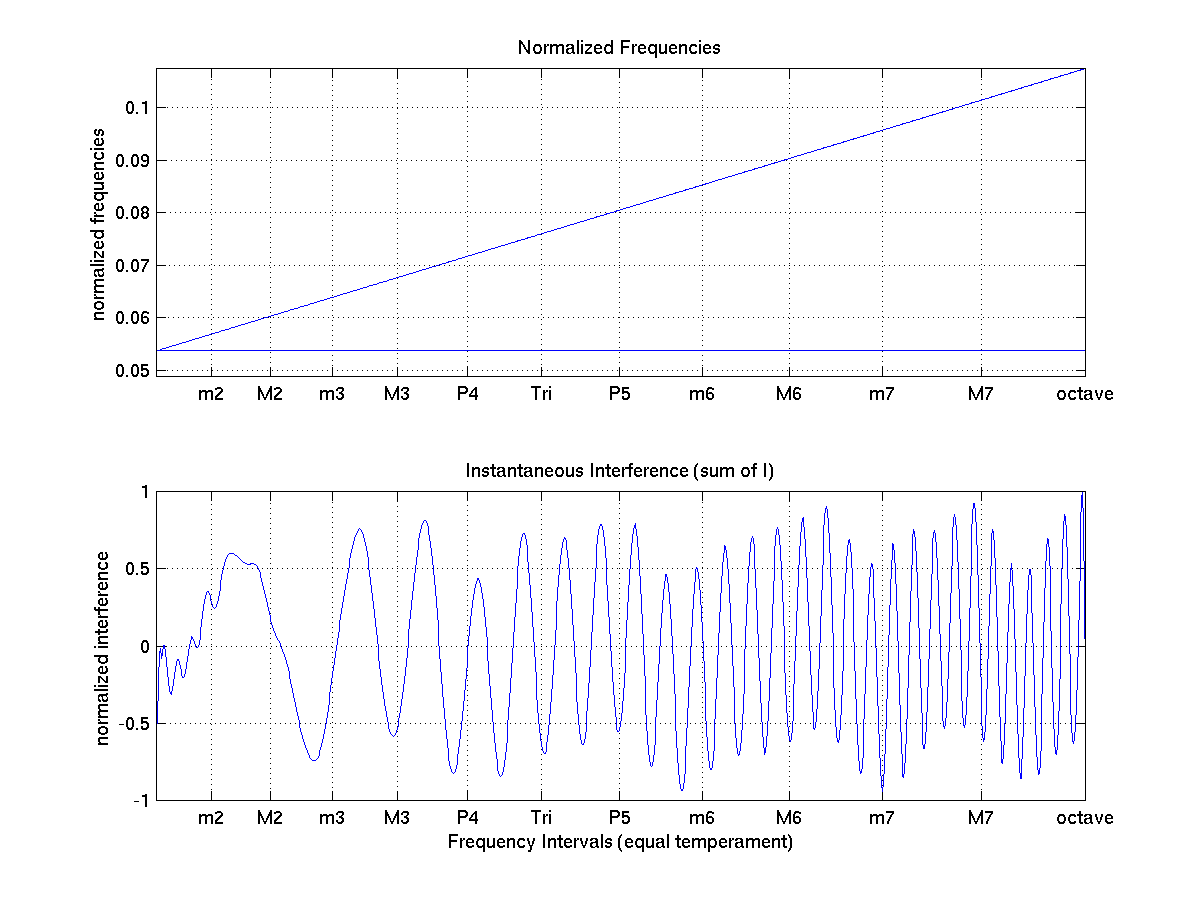
\includegraphics[width=16cm, height=14cm]{sumIequal}
  \end{center}
%  the sum of interferences at each point in time; the time 
\end{slide}
}

\ifthenelse{\boolean{nofigures}}{}{
\begin{slide}%%% Slide
$\I_x(t)$ with time axes delimited by just (top)\\ 
and Pythagorean (bottom) tunings.
%table gives corresponding frequency ratios. 
\begin{center}
  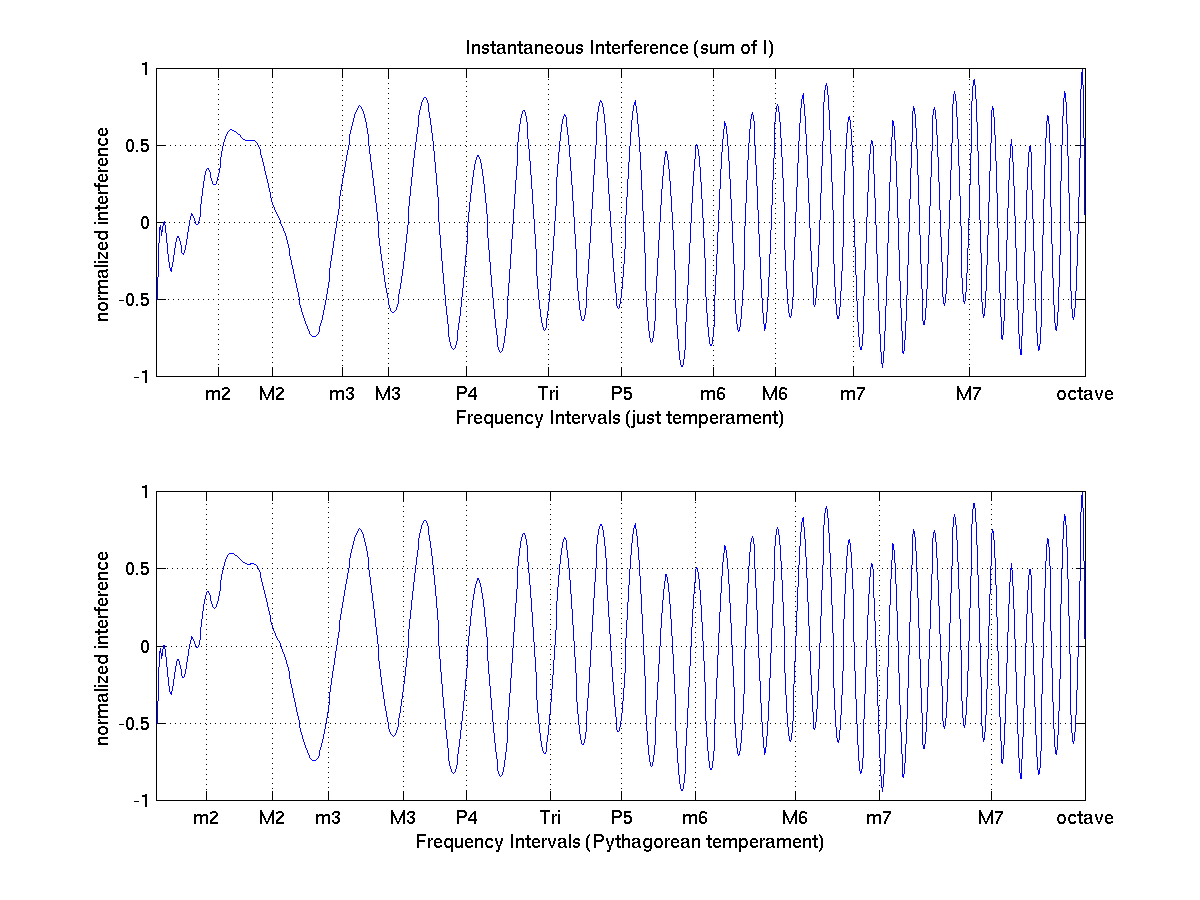
\includegraphics[width=14cm, height=10cm]{sumIjust}
\end{center}
%Instantaneous interference for just (top), and \\
%Pythagorean (bottom) tunings.
\end{slide}
}

\ifthenelse{\boolean{notable}}{}{
\begin{slide}%%% Slide
Frequency ratios for horizontal axes.
  \begin{center}
\begin{tabular}{l|r|r|r}
Name & Just & Pythagorean & Equal\\
\hline
m2 &16/15& 256/243& $2^{1/12}$\\
M2 & 9/8 & 9/8& $2^{2/12}$\\
m3 &6/5 & 32/27& $2^{3/12}$\\
M3 &5/4 & 81/64& $2^{4/12}$\\
P4 &4/3 & 4/3& $2^{5/12}$\\
Tritone &64/45 & 729/512& $2^{6/12}$\\
P5 &3/2 & 3/2 & $2^{7/12}$\\
m6 &8/5&128/81& $2^{8/12}$\\
M6 & 5/3& 27/16 & $2^{9/12}$\\
m7 & 7/4& 16/9 & $2^{10/12}$\\
M7 & 15/8& 243/128 & $2^{11/12}$\\
octave& 2 & 2 & $2^{12/12}$
\end{tabular}
\end{center}
\end{slide}
}


%\begin{center}{\tt \underline{OBSERVATIONS}}\end{center}
%$\cdot$ 3 tuning systems have roughly same P5\\
%$\cdot$ P5 corresponds to local minimum of $\I_x(t)$\\
%$\cdot$ other significant intervals correspond to local minima\\
%(e.g.~M3 and tritone)


\begin{slide}%%% Slide
$\I_x(t)$ essentially sums $I_x(t,\nu)$ over $\nu$.\\
%Since $I_x(t,\nu)$ is a measure of interferences among
%signal components centered at $t$ as well as those centered at times
%surrounding $t$, it might seem as though the function $\I_x(t)$ accounts for
%melodic context.  
%However, note that
%\[
%\I_x(t) =\sum_{m,n}
%      \langle R^mx,g_{\gamma_m}\rangle \langle R^nx,g_{\gamma_n}\rangle^*
%        g_{\gamma_m}(t) g^*_{\gamma_n}(t)
%\]
%by equation~(\ref{eq:intWV}).
$\Rightarrow$ measures interferences only at time $t$.
%Still, as the results for our simple example show, it may provide a useful
%point-wise dissonance characterization of a signal.

{\bf 2nd Dissonance Measure:}\\
Fourier transform the interference energy.
\[  
\I_x(t,\tau) = \int I_x(t,\nu)e^{i2\pi\nu\tau}\; d\nu  
\]
\[
= \sum_{m, n}\langle R^mx,g_{\gamma_m}\rangle \langle R^nx,g_{\gamma_n}\rangle^* 
\phi_{g_{\gamma_m}g_{\gamma_n}}(t,\tau)
\]

$\I_x(t,\tau)$ leads to measure of interference
among signal components at different points in time.

%Recall,
%\[
%\phi_{g_{\gamma_m}g_{\gamma_n}}(t,\tau) 
%= g_{\gamma_m}\tpull g^*_{\gamma_n}\tpush
%\]
\end{slide}

\begin{slide}%%% Slide
Measure interferences separated by up to
$\tau_0$ units of time:
\begin{align*}
\I_x^{\tau_0}(t) &= \int_0^{\tau_0} \I_x(t,\tau)\; d\tau\\
\\
&=\sum_{m, n} \langle R^mx,g_{\gamma_m}\rangle \langle
                      R^nx,g_{\gamma_n}\rangle^* \\
&\quad \times \int_0^{\tau_0} g_{\gamma_m}\tpull g^*_{\gamma_n}\tpush\;d\tau
\end{align*}

$\tau_0$ determines maximum time interval across which to measure interferences.
\end{slide}

\ifthenelse{\boolean{nofigures}}{}{
\begin{slide}%%% Slide
$\I_x^{\tau_0}$ for two values of $\tau_0$.
  \begin{center}
  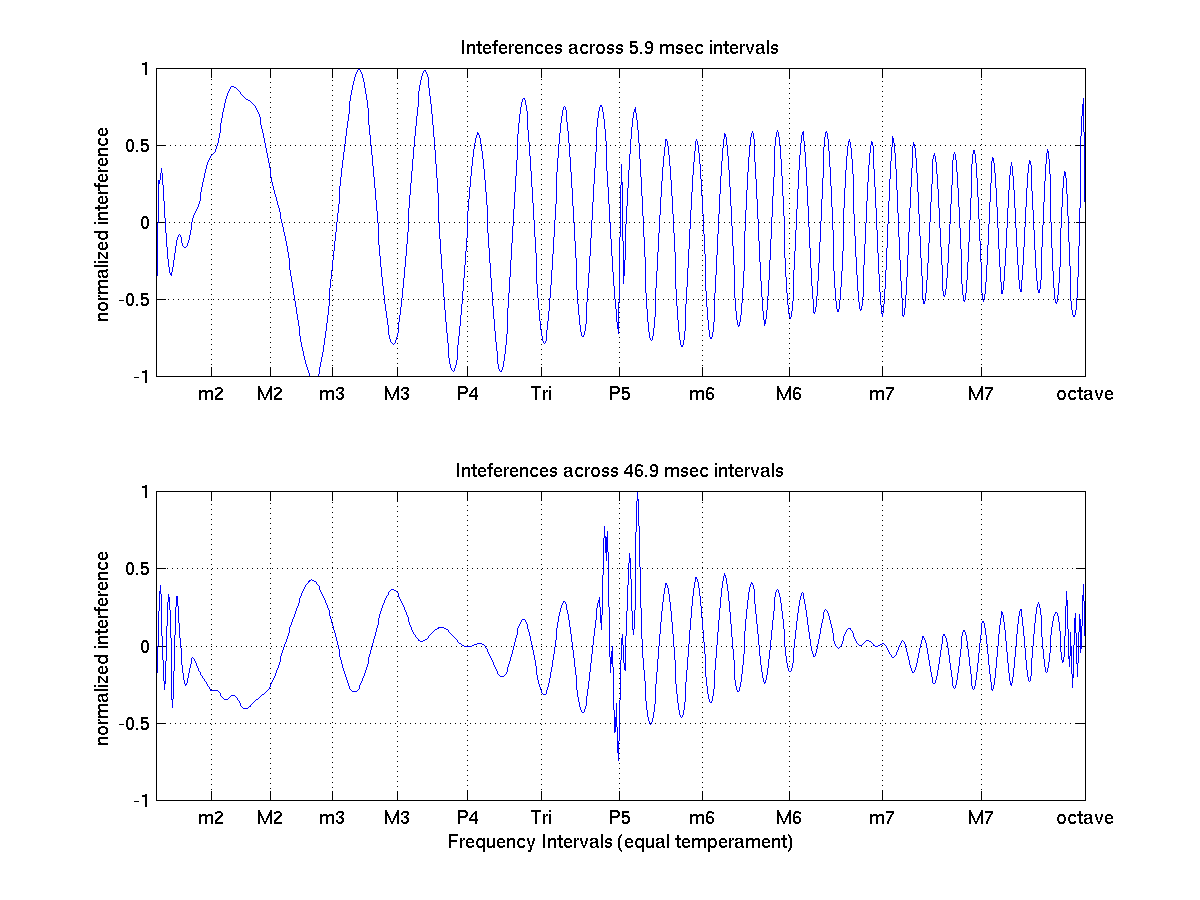
\includegraphics[width=14cm, height=10cm]{IcorrEqual}
\end{center}
$\I_x^{\tau_0}$ for $\tau_0 = 6$ milliseconds (top), and \\
$\tau_0 = 47$ milliseconds (bottom).  
%Taken as a measure of dissonance, figures indicate that dissonance is maximal 
%when the ratio approaches the perfect fifth and minimal once it reaches the
%perfect fifth.  
\end{slide}
}

\begin{slide}%%% Slide
{\bf General Dissonance Measure:}\\
Put distribution $\mu$ on domain of time intervals; $\mu$
describes relative importance of interference among time intervals.\\
Define 
\begin{equation*}
\I_x^{\mu}(t) = \integral \I_x(t,\tau)\; d\mu(\tau)
\end{equation*}

1st and 2nd measures are special cases. 
%$\mu$ uniform with width $\tau_0$,
\[
\I_x^{\tau_0} \; \leftrightarrow \; d\mu(\tau) =
\chi_{[0,\tau_0)}(\tau)\;d\tau
\]
%where $\chi_{[0,\tau_0)}(\tau)$ is the characteristic function, equal to 1 when
%$\tau \in [0,\tau_0)$ and 0 elsewhere. 
%Therefore, $\mu$ assigns equal importance to interferences among components
%separated by at most $\tau_0$ units of time, and zero importance to
%interferences among components separated by more than $\tau_0$
%units. 
\[
\I_x \; \leftrightarrow \; \mu(\tau) =\delta(\tau)
\]
\end{slide}

\begin{slide}%%% Slide
\begin{center}{\tt \underline{SUMMARY \& CONCLUSIONS}}\end{center}
\begin{itemize}
\item defined ``interference energy'' function $I_x(t,\nu)$ to be sum of
cross terms in atom expansion of $W_x$.
\item defined measures $\I_x$ and $\I_x^{\tau_0}$ quantify interference among
signal components at points and over intervals, resp.
\item defined more general measure $\I_x^{\mu}$ employing a distribution
on the domain of time differences between signal components.  
\item observed interesting behavior for simple composition of pure tones.  
%\item as yet unclear how useful, as measures of dissonance,  %is the information provided by 
%are such functions.  
\end{itemize}
\end{slide}
\begin{slide}
\begin{center}{\tt \underline{FUTURE WORK}}\end{center}
\begin{enumerate}
\item optimize atomic decomposition algorithm \\(e.g.~employ better MP)
\item experiment with real music examples
\item experiment with various distributions $\mu$
\end{enumerate}
\end{slide}

\end{document}


%%%%%%%%%%%%%%%%%%%%%%%%%%%%%%%%%%%%%%%%%%%%%%%%%%%%%%%%%%%%%%%%%%%%%%%%%%

\begin{slide}%%% Slide
\begin{center}{\tt \underline{}}\end{center}
\end{slide}
\begin{slide}%%% Slide
\begin{center}{\tt \underline{}}\end{center}
\end{slide}
\begin{slide}%%% Slide
\begin{center}{\tt \underline{}}\end{center}
\end{slide}
\begin{slide}%%% Slide
\begin{center}{\tt \underline{}}\end{center}
\end{slide}


%%%%%%%%%%%%%%%%%%%% BEGIN: EXAMPLE %%%%%%%%%%%%%%%%%%%%

\begin{slide}%%% Slide
\begin{center}{\tt \underline{EXAMPLE}}\end{center}
%An example will help describe the structure of the 
%cross terms of the \WT\ 
Consider atom $x(t)$ centered at $t=0$. \\%\cite{Flandrin:1999}. 
Construct two time-frequency shifted versions:

For $\a = (a_1,a_2), \b = (b_1,b_2)$,
\begin{alignat*}{2}%\[
\alpha\; x_\a(t)&=\alpha \;x(t-a_1)\; e^{i2\pi a_2t}, \quad \alpha\; &\geq0\\
\beta\; x_\b(t)&=\beta\;x(t-b_2)\;e^{i2\pi b_2t}, \quad \beta &\geq 0
\end{alignat*}%\]
\end{slide}
\begin{slide}
The composite signal $x_\a(t)+x_\b(t)$ has WVT
\[
  \W_{x_\a+x_\b}(t,\nu) 
    = \W_{x_\a}(t,\nu)+\W_{x_\b}(t,\nu) + I_{x_\a x_\b}(t,\nu)
\]
\\
with terms
\begin{align*}
\W_{x_\a}(t,\nu) &= \alpha^2\W_x(t-a_1,\nu-a_2),\\
\W_{x_\b}(t,\nu) &= \beta^2\W_x(t-b_1,\nu-b_2),\\
  I_{x_\a x_\b}(t,\nu)&=
    2\alpha \beta \W_x(t-t_m,\nu-\nu_m)\\
    & \times \cos\left\{2\pi \left[(t-t_m)\Delta\nu 
               -(\nu-\nu_m)\Delta t \right]\right\}
\end{align*}
where
\begin{alignat*}{2}
  t_m    &= \frac{a_1+b_1}{2}, \quad 
  \nu_m &&= \frac{a_2+b_2}{2}\\
  \Delta t    &= a_1-b_1,\quad
  \Delta \nu &&= a_2-b_2
\end{alignat*}
\end{slide}
\begin{slide}
\begin{center}{\tt \underline{OBSERVATIONS}}\end{center}
Energy of $\W_x$ centered at $(0,0) \; \Rightarrow$\\
$\cdot$ energy of $\W_{x_\a}$ centered at $\a = (a_1,a_2)$\\
$\cdot$ energy of $\W_{x_\b}$ centered at $\b = (b_1,b_2)$\\
\\
\def\lab{\ensuremath{\ell}}
Let \lab\ denote the line joining $\a$ and $\b$; \\
$I_{x_\a x_\b}(t,\nu)$ is an
oscillating wave form with \\
%\begin{itemize}\item
$\cdot$ center at geometric midpoint of \lab\\
%between $\a $ and $\b$.\\
$\cdot$ frequency proportional to length of \lab\\
%$\sqrt{\Delta \nu^2 + \Delta t^2}$ of \lab.\\
%between $\a $ and $\b$.\\
$\cdot$ direction perpendicular to \lab
%line joining $\a $ and $\b$.
%\end{itemize}
% $(t_1,\nu_1)$ and $(t_2,\nu_2)$.
\end{slide}

%%%%%%%%%%%%%%%%%%%% END: EXAMPLE %%%%%%%%%%%%%%%%%%%%


\begin{slide}%%% Slide 
\begin{align*}
  \W_{x+y}(t,\nu) &= \W_x(t,\nu) + \W_y(t,\nu)\\
      \quad &+ \W_{xy}(t,\nu) +\W_{yx}(t,\nu)
\end{align*}
Define the ``interference term'' by
\[I_{xy}(t,\nu) = \W_{xy}(t,\nu) +\W_{yx}(t,\nu)\]
%Then\[\W_{x+y}(t,\nu) = \W_x(t,\nu) + \W_y(t,\nu)+I_{xy}(t,\nu) \]
\end{slide}
\def\a{\mathbf{a}}
\def\b{\mathbf{b}}


